恭喜你已经成功安装了 Ubuntu 双系统。作为新手，想来你在刚刚的安装过程中一定很小心，毕竟谁也不想刚装好就出什么差错。不过在后续的工作中，我们还会安装各种各样的软件包、配置各种各样的环境，如果不小心配错了东西，轻则程序找不到，重则系统无法正常工作（简称寄了）。这时候就需要根据问题进入恢复选项、修正配置，实在处理不了才考虑重装。

当然，我们肯定不愿意每次都从头再来，所以很有必要学会备份（Backup）：在大改环境之前存个档，出问题时才有机会回到改动之前。不过系统配置和你写的代码不一定保存在同一份备份里，下面我们先把这个范围分清楚，再试一次恢复。存档到底能不能读，也要试过才知道。
\label{sec:system-backup}

\subsubsection{Timeshift 系统快照}
Timeshift 可以给系统文件和设置制作快照（Snapshot），你可以把它想成给系统照一张相，后来配环境出了问题，再按这张相恢复。操作并不复杂，比事后重新配一遍省事得多；不过相机拍到了什么，还是要看你设置的范围，不是按一下就把整台电脑都保存了。
\begin{note}
\textbf{Timeshift 默认排除个人文件。}源码、照片、数据集要另做备份；快照放在同一块物理盘上，也无法抵御这块盘损坏。恢复会把所选系统文件还原到快照状态，期间的新配置可能被覆盖。先备份个人数据和当前配置，确认目标系统与快照，再恢复。官方说明见 \url{https://github.com/linuxmint/timeshift}。
\end{note}
\Needspace{8\baselineskip}
\begin{example}[创建并核对系统快照]
首先在 Ubuntu 中安装 Timeshift，然后从应用菜单点击它的图标，或者在终端里输入最后一条命令，进入配置向导：


\Needspace{7\baselineskip}
\begin{tbash}
sudo apt update
sudo apt install timeshift
sudo timeshift-launcher
\end{tbash}


进入向导后，首先选择快照类型。我们前面安装的是一般的 ext4 系统，选 RSYNC 即可；它借助 rsync 与硬链接保存文件，未变化的内容可以共享。BTRFS 则利用文件系统本身的快照，但要求受支持的子卷布局，不是看到磁盘格式叫 Btrfs 就一定能用。

然后选择保存快照的位置，按磁盘型号和容量认清目标，并确认它有足够空间、支持 Linux 权限和硬链接。有条件的话，我们可以用另一块盘来保存，这样原来的盘坏了，备份才不至于跟着一起消失。自动备份页面可以选择每月、每周、每天等计划，旁边的数量表示保留多少份；旧快照会按保留策略清理，所以先想好自己要留多久，不必把所有选项都勾上。

接下来读清“用户主目录”和“筛选”页：哪些文件包含在内，哪些排除在外。确认范围后完成向导，点击“创建”，等快照制作完成。我们再用下面的命令查看列表：


\Needspace{5\baselineskip}
\begin{tbash}
sudo timeshift --list
\end{tbash}


列表里应该能找到这次的时间、标签和注释，创建过程也不应该有失败提示。到这里就有了一份系统快照，不过个人代码和数据仍要按照前面的提醒另做备份。完成初始配置后，你也可以直接在命令行创建手动快照，通用形式为 \texttt{timeshift --create [选项]}，比如：


\Needspace{6\baselineskip}
\begin{tbash}
sudo timeshift --create --comments "before-training" --tags O
sudo timeshift --list
\end{tbash}


这里的 \texttt{--comments} 用来写说明，\texttt{--tags O} 表示按需创建。设备选择沿用你刚刚核对过的配置，我们不用照抄别人的磁盘名。
\end{example}
\begin{figure}[H]
\centering
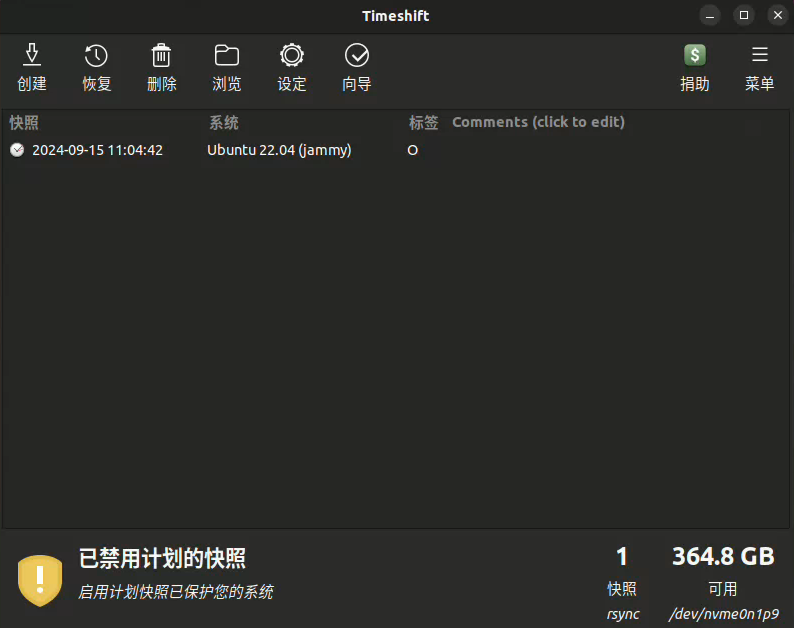
\includegraphics[width=0.8\textwidth]{restore1.png}
\caption{Timeshift 列表：核对时间、系统版本与快照数量；截图不是本次创建结果}
\label{fig:restore1}
\end{figure}

\textbf{接下来我们看看怎样恢复。}如果系统还能正常打开桌面，就启动 Timeshift，选择刚刚核对过的快照，点击“恢复”。这里要特别留意目标设备页：根分区、EFI 分区等映射指的是要恢复到哪里，不只是备份存在哪里。先确认当前文件已经另做备份、目标系统也选对了，再读一遍最终变更摘要，确认后继续。恢复结束后重启，看看被恢复的配置是否回到原来的内容，个人文件是否仍在。
\begin{figure}[H]
\centering
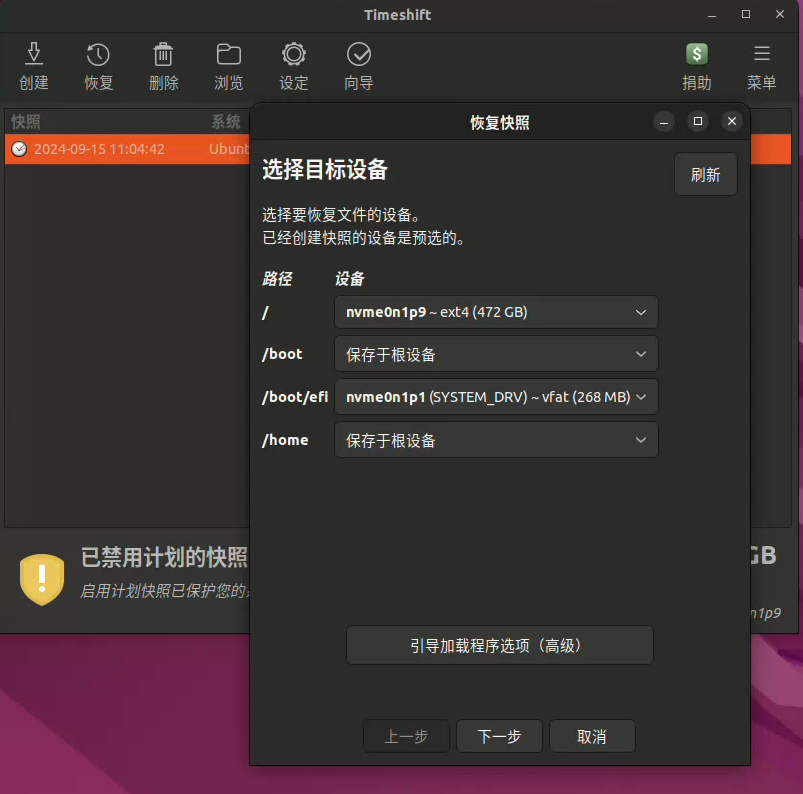
\includegraphics[width=0.75\textwidth]{restore2.png}
\caption{恢复目标选择页：确认的是目标分区，不只是备份保存位置}
\label{fig:restore2}
\end{figure}
如果图形化桌面已经打不开，但还能进入 TTY，可以先运行 \texttt{timeshift --help} 看当前版本的用法，再通过 \texttt{timeshift --restore} 进入交互恢复。如果连系统都进不去了，这时候之前保存的“数字生命”就派上用场了：从 Live U 盘进入 Try Ubuntu，安装 Timeshift，再选择备份所在的设备和要恢复的目标系统。不要为了让命令少问几句，就照抄不明理由的 \texttt{--skip-grub} 跳过引导处理。

我们练习恢复时，优先用虚拟机或可以重建的练习系统：快照前保存一份练习配置，然后改动它，再恢复，看看内容是不是真的变回来了。不用为了交练习把自己正在使用的系统盲目回档；如果暂时没有练习系统，就先记下创建结果和恢复计划，把\textbf{实际系统恢复留作待验证}，等有合适环境再补上。
\begin{exercise}\label{ex:v1-snapshot}
创建一个带注释的快照，记录列表、保存设备和排除范围。说明哪些个人文件仍需另备份；在可重建系统中完成一次配置恢复并记录前后内容，没有该环境时明确待验证项。
\end{exercise}

\subsubsection{文件归档与恢复：先在小目录里练}
\label{sec:archive-backup}
Timeshift 帮我们保存系统状态，那自己写的代码和配置又怎样备份呢？接下来介绍 \texttt{tar}，它可以把多个文件打成归档（Archive），配合 gzip 压缩后，常见的扩展名就是 \texttt{.tar.gz}。这样我们就能把一个目录里的内容打包带走，再解到另一个地方。

不过 tar 归档不是整块磁盘的扇区镜像，它没有自动保存 GPT、EFI 引导状态，也不能保证正在写入的文件前后一致。直接“把 / 打包，再解压到 /”还可能覆盖真实系统，对新手来说既难验证又难补救。所以这里我们先在一个小目录里练清楚备份和恢复的过程；如果以后需要迁移整个系统，再单独准备完整的恢复方案。

通用形式为 \texttt{tar -czf 归档文件 -C 起始目录 要保存的相对路径}；恢复用 \texttt{tar -xzf 归档文件 -C 目标目录}。\texttt{-c} 创建、\texttt{-x} 解包、\texttt{-z} 使用 gzip、\texttt{-f} 指定归档文件，\texttt{-C} 先切换基准目录，\texttt{-t} 列内容，\texttt{-v} 显示详细过程；\texttt{-p} 在解包时尽量恢复权限，不是提高压缩完整性。
\Needspace{8\baselineskip}
\begin{example}[备份、损坏、恢复与额外文件]
我们先造一个只有配置文件的小环境，备份它，再故意把恢复目录里的配置改坏，最后试着读档。在 Bash 终端一次执行下列命令即可，\texttt{mktemp -d} 会创建独立的临时目录，下面的覆盖都发生在这个实验目录里，不需要 sudo。

\begin{tbash}
lab=$(mktemp -d)
mkdir -p "$lab/source" "$lab/restored"
printf 'camera=ready\n' > "$lab/source/config.txt"
tar -czf "$lab/backup.tar.gz" -C "$lab/source" .
tar -tzf "$lab/backup.tar.gz"
printf 'camera=broken\n' > "$lab/restored/config.txt"
printf 'keep me\n' > "$lab/restored/extra.txt"
tar -xzf "$lab/backup.tar.gz" -C "$lab/restored"
cmp "$lab/source/config.txt" "$lab/restored/config.txt"
cat "$lab/restored/config.txt" "$lab/restored/extra.txt"
printf 'lab=%s\n' "$lab"
\end{tbash}

运行后，归档列表里应该能看到 \texttt{./config.txt}。\texttt{cmp} 是比较文件内容的命令，成功时没有输出，退出码为 0；最后两行文件内容应该是 \texttt{camera=ready} 和 \texttt{keep me}。配置从 broken 变回 ready，说明同名文件确实恢复了，不过后来添加的 extra.txt 还在。也就是说，\textbf{解包不等于让整个目标目录精确回到旧状态}，这个“读档”不会自动把后来多出来的文件删掉。
\end{example}
\begin{note}
\texttt{tar -x} 会覆盖目标中的同名文件。真实备份先解到新的空目录，检查内容和权限，再决定怎样合并。不要对不可信归档用 root 解包；不要把 \texttt{-C /} 当作通用恢复命令。tar 的非零退出码也不能一律忽略：读失败、文件变化或空间不足时，检查 stderr 并重新验证归档。
\end{note}
\begin{exercise}\label{ex:v1-tar-options}
解释 \texttt{-c/-x/-z/-f/-C/-t/-p} 的作用，实际运行目录恢复实验。修改一个源文件后重新备份到\textbf{另一个归档名}，解到新的空目录并用 \texttt{cmp} 验证，说明为何额外文件不会自动消失。
\end{exercise}
\begin{conclusion}
Timeshift 主要保护系统配置，tar 适合文件归档；两者的有效性都依赖恢复验证。备份范围、保存介质和恢复目标要一起记。系统快照不代替个人数据备份；文件归档不等于完整磁盘镜像，解包也不会删除后来新增的文件。
\end{conclusion}
